\documentclass{article}
\usepackage{graphicx}
\begin{document}
\section{Discrete Cmac}
\subsection{Description}
\subsection{Results}
  \paragraph{Generalization Vs Convergence:}
   Clearly from the graphs shown below,it can be noted that  
  as the generalization number increases, the model has a hard time converging.This can
  be attributed to the fact that the generalization number,g indicates to a degree the similarity
  between tasks. As the g increases, unrelated tasks are grouped as similar and the model tends
  to overfit. Ideally, g is chosen so that tasks which are related have similar value whiles tasks
  which are different have clear cut distinct values. 
  \begin{figure}[h!]
    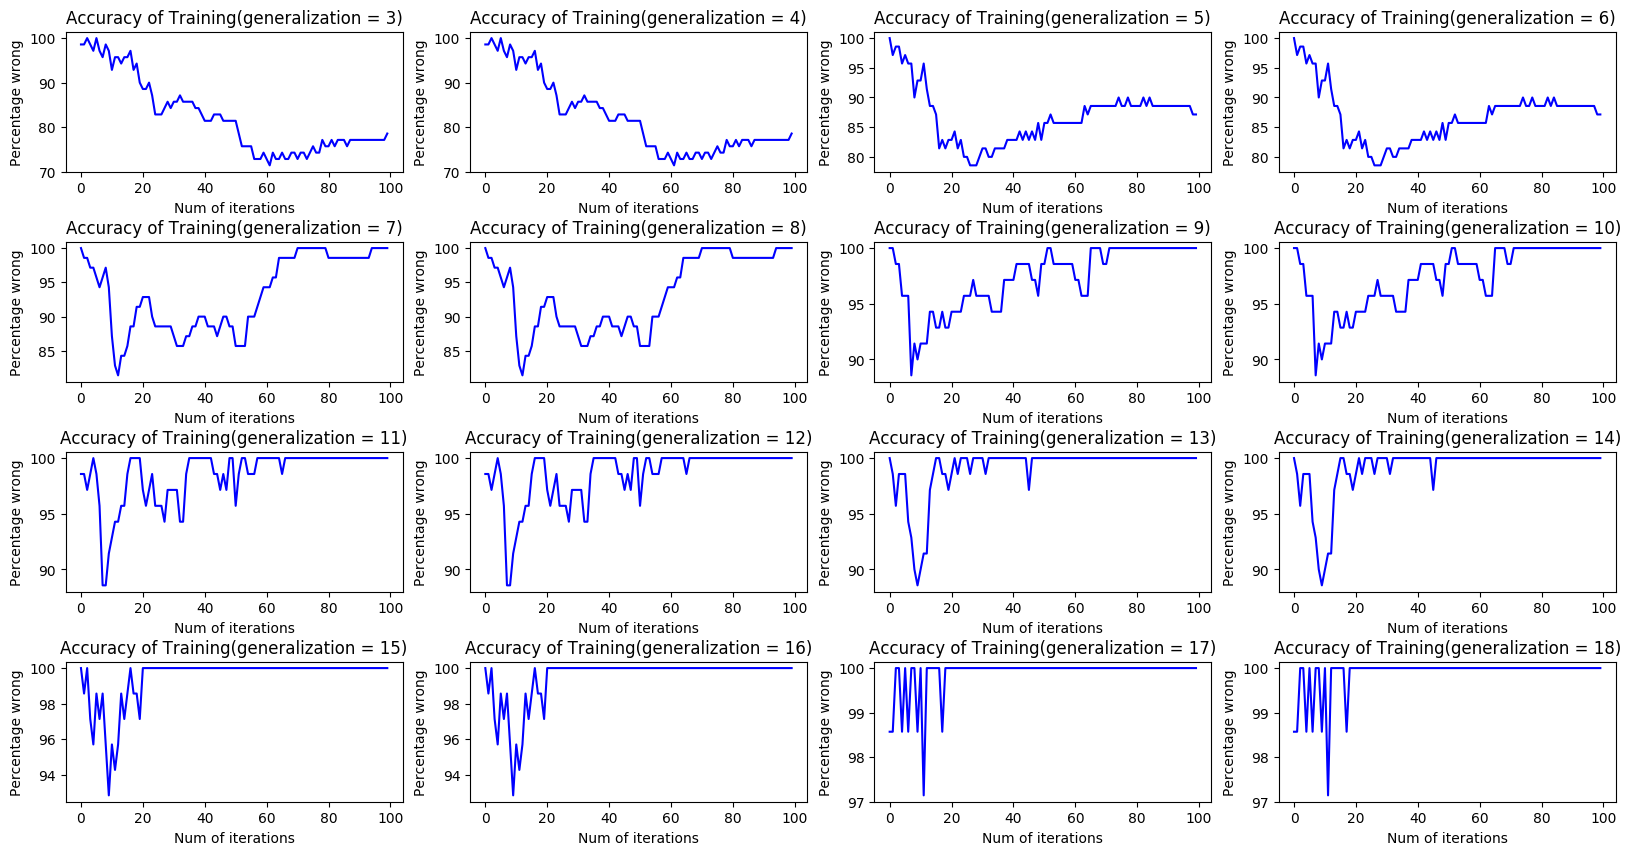
\includegraphics[scale=0.35]{./Results/convergenceVsgeneralization.png}
  \end{figure}

  \paragraph{Accuracy:}
    Below is a graph that depicts the accuracy of the Discrete Cmac. After running a couple of times, it can 
    be noted that the accuracy hovers between 70-80\%
  \begin{figure}[h!]
    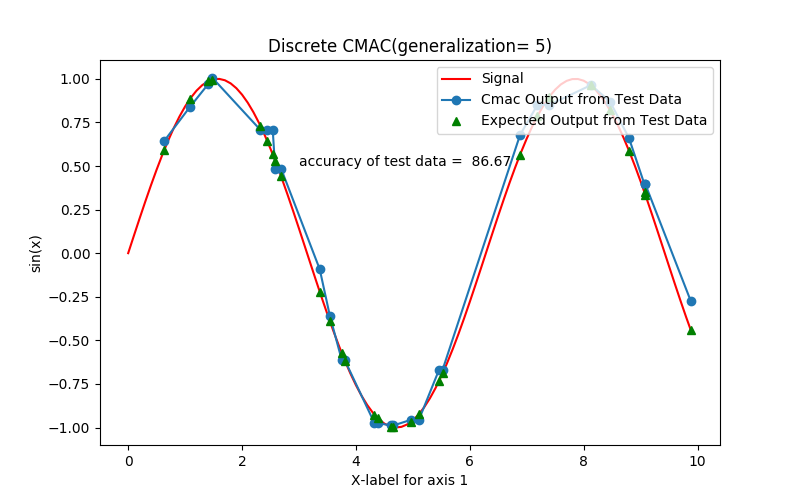
\includegraphics[scale=0.7]{./Results/discreteAccuracy.png}
  \end{figure}
\newpage 
\section{Continous Cmac}
\subsection{Description}
\subsection{Results}
  \paragraph{Accuracy:}
    Below is a graph that depicts the accuracy of the Continous Cmac. After running the the code a couple of times, it can
    be noted that the accuracy hovers between 40-60\%
  \begin{figure}[h!]
     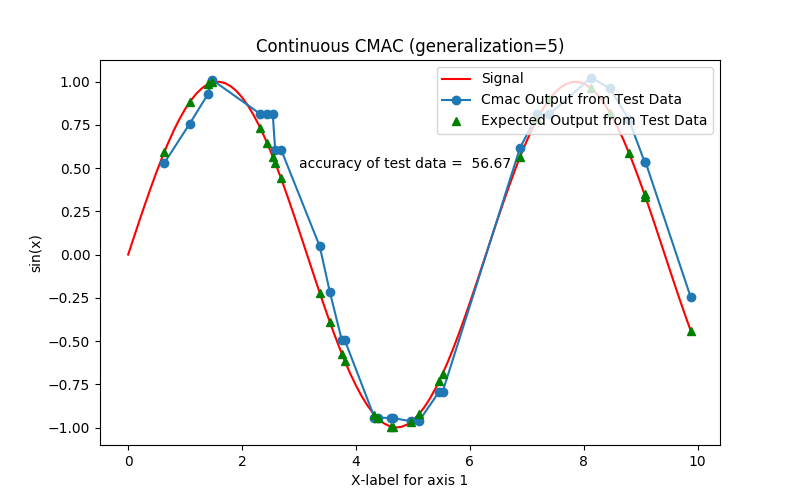
\includegraphics[scale=0.65]{./Results/continousAccuracy.png}
  \end{figure}
  \paragraph{Discrete Vs Continous Cmac:}
  For the same parameters used in training the Discrete Cmac(generalization number, number of iterations in training,accuracy used in training,learning rate), it can be noted that the continous Cmac has a significant drop in accuracy as the model clearly seems to overfit.This is because the continous cmac slides over more weights. Therefore, although a generalization number of 5 is used, more than 5 weights are changed during each update and this means that more inputs are categorized as similar and that is undesirable. To rectify this the generalization number can be reduced and number of iterations increased to improve perfomance.   
\newpage
\section{Recurrent Networks}
\end{document}


